\documentclass[a4paper, 12pt, titlepage]{article}

%
% Importering av pakker
%
\usepackage[latin1]{inputenc}
\usepackage[T1]{fontenc, url}
%\usepackage{babel}
\usepackage{textcomp}
\usepackage{amsmath, amssymb}
\usepackage{amsbsy, amsfonts}
\usepackage{graphicx, color}
\usepackage{parskip}
%
% Parametere for inkludering av kode fra fil
%
\usepackage{listings}
\lstset{language=python}
\lstset{basicstyle=\ttfamily\small}
\lstset{frame=single}
\lstset{keywordstyle=\color{red}\bfseries}
\lstset{commentstyle=\itshape\color{blue}}
\lstset{showspaces=false}
\lstset{showstringspaces=false}
\lstset{showtabs=false}
\lstset{breaklines}

%
% Layout
%
\topmargin = -50pt
\oddsidemargin = -30pt
\textheight = 710pt
\textwidth = 490pt

%
% Definering av egne kommandoer og miljøer
%
\newcommand{\dd}[1]{\ \text{d}#1}
\newcommand{\f}[2]{\frac{#1}{#2}} 
\newcommand{\beq}{\begin{equation*}}
\newcommand{\eeq}{\end{equation*}}
\newcommand{\beqq}{\begin{equation}}
\newcommand{\eeqq}{\end{equation}}
\newcommand{\bt}[1]{\textbf{#1}}
\newcommand{\n}{\newline}
\newcommand{\pa}{\partial}
%
% Navn og tittel
%
\author{Candidate number 16}
\title{FYS3150 - Project 5}

\begin{document}
 \maketitle
 \newpage
 
 \begin{section}*{Introduction}
  This project will be about solving the diffusion equation in both 1 and 2 spacial dimensions both 
  analytically and numerically. This equation is widelly used in both thermodynamics, statistical physics and
  quantum mechanics to name a few. Therefore, I will use different schemes, and compare it with the analytical
  solutions to find the most efficient and stable solution. In this specific case, I simulate
  the concentration of neurotransmitters between two nerve cells, neurons. This concentration can be simulated
  by the diffusion equation. 
  
  A few notes: I have made mpg movies of the solutions, but unfortunatly they could not be delivered on a 
  printed PDF. I have yet to receive feedback on project 4, so I haven't been able to confirm that what I did
  in that project is correct. The movies can be found at https://github.com/wholmen/FYS3150-Project-5 in
  the folder Movies for Project 5.
 \end{section}

 \begin{section}*{1+1 dimensional problem}
  First I will look at the 1+1 dimensional problem. That means one spacial dimension, x, and one time 
  dimension. In this simulation we set the amount of neurotransmitters equal to one at the presynaptic,
  $x=0$. This will not change throughout the simulations, because the axon produces the neurotransmitters.
  The postsynaptic absorbs all the neurotransmitters, so the concentration will always be 0 at $x=1$. 
  The concentration throughout the cleft is given by the diffusion equation:
  \beq D\frac{\pa^2 u}{\pa x^2} = \frac{\pa u}{\pa t} \eeq
  In our case, we set $D=1$. 
 
  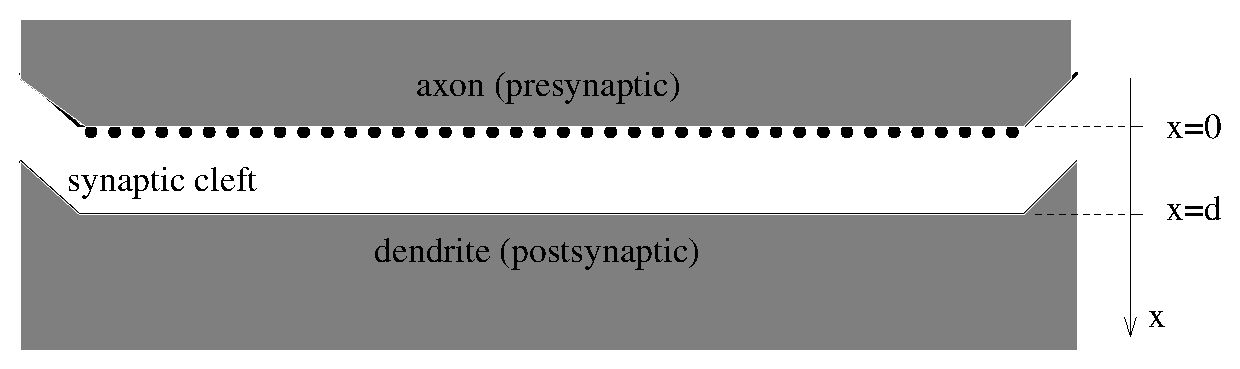
\includegraphics[width=0.8\textwidth]{build-main-Desktop-Debug/synaptic_cleft.eps}{\centering}
 
 \end{section} 
 
 \begin{section}*{1+1 dimensional problem, analytical solution}
 
    We want the boundary conditions equal to $0$ at both $x=0$ and $x=1$, so we define a new function 
    \beq v(x,t) = u(x,t) - u_s(x,t) \eeq
    and solve the diffusion equation for this function. This equation can be solved by separation of
    variables. Setting $v(x,t) = X(x)T(t)$ gives:
    \beq \f{\pa T}{\pa t} \f{1}{T(t)} = \f{1}{X(x)} \f{\pa ^2 X}{\pa x^2} = -\lambda ^2\eeq
    The soltion for the time equation is \beq T(t) = e^{-\lambda ^2 t} \eeq while the spacial solution is
    \beq X(x) = Asin(\lambda x) + Bcos(\lambda x) \eeq
    By the boundary conditions $v(0,t) = v(1,t) = 0$ we see that $B = 0$ and that $\lambda = n\pi$. 
    So we get \beq v(x,t) = \sum_{n=1}^{\infty} C_n sin(n\pi x) e^{-n^2\pi ^2 t} \eeq
    The initial condition is given on the form $Ax + b$, so $u_s(x) = 1-x$ fullfills the boundary conditions. 
    We have defined $v(x,t) = u(x,t) - u_s(x)$ so $u(x,t) = v(x,t) + u_s(x)$, 
    \beq u(x,t) = 1 - x + \sum_{n=1}^{\infty} C_n sin(n\pi x)e^{-n^2\pi ^2 t}  \eeq 
    
    To find the $C_n$s, I solve the equation for time equal to 0. I know that $u(x,0) = 0$ for $0<x<1$, so
    \beq v(x,0) = \sum_{n=1}^{\infty} C_n sin(n\pi x) = x - 1 \eeq
    Using the fourier expansion we see that \beq C_n = \f{-2}{\pi n} \eeq and we get the full solution
    
    \beq u(x,t) = \sum_{n=1}^{\infty} \f{-2}{\pi n} sin(n\pi x) e^{-n^2\pi ^2 t} + x - 1 \eeq
    
    Which we see approaches the steady state solution after some time. Here I used 100 points along the 
    x-axis and i let the sum go from $n=1$ to $n=15$. The right plot is the first 6 analytic solutions. As time passes, the solution moves more 
    and more towards the steady state solution.
    
    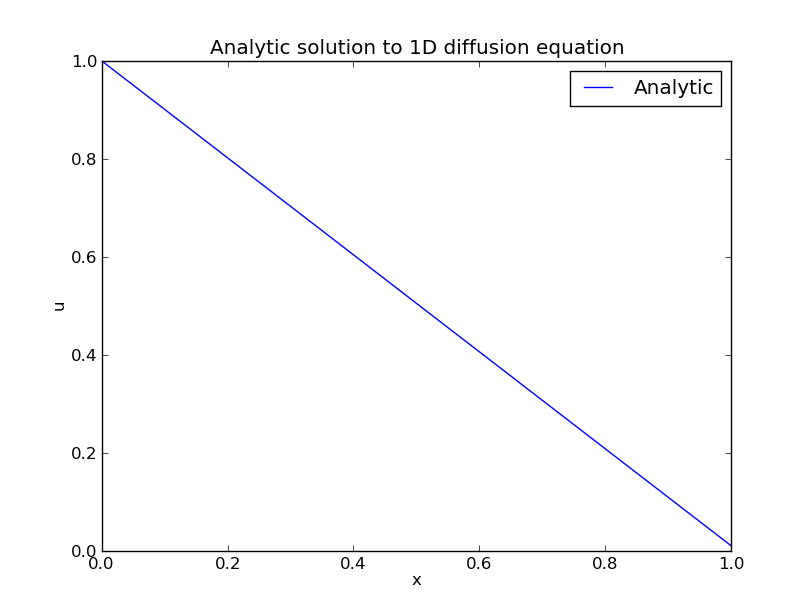
\includegraphics[width=0.55\textwidth]{build-main-Desktop-Debug/Analytic_1d.png}
    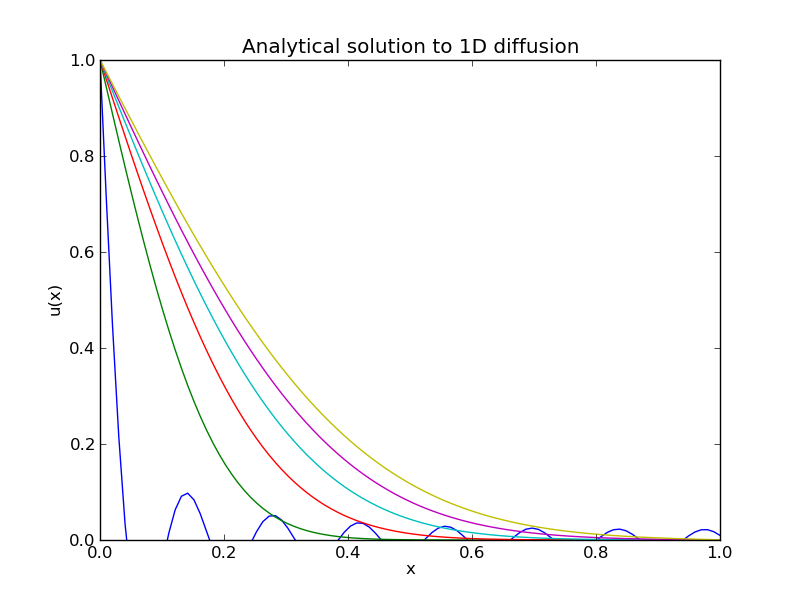
\includegraphics[width=0.55\textwidth]{build-main-Desktop-Debug/Analytic_1d_first6.png}
    
     
 \end{section}
 \begin{section}*{1+1 dimensional, numerical solution}
  \begin{subsection}*{Markov Chains}
  In this project I will solve the 1+1 dimensional diffusion equation by Monte Carlo methods using Markov 
  Chains. I will simulate the diffusion equation by programming the following random walk steps: \par
  1. Set initial number of particles, $N_0$, that start at $x=0$. This number will be conserved for $x = 0$
  throughout the whole simulation. \n
  2. Set up a vector, $u$, that contain positions of each individual particle. The positions will be split
  up into $Nx$ different bins with width $dx$. \n
  3. For each particle, draw a random number, $r$. If $ r < 0.5 $ then $ pos_{new} = pos_{old} - l_0$
     else $pos_{new} = pos_old + l_0$. \n
  4. If a particle moves beyond $x=1$, remove particle. \n
  5. If a particle moves from $x=0$, add a new at $x=0$ to maintain $N_0$. In addition: If the move is 
     negative, remove particle from vector. \n
  6. Repeat 2-5 for all time steps until final time is reached. \par
  I will implement two different algorithms. The first algorithm will have constant steplength
  \beq l_0 = \sqrt{2\Delta t} \eeq 
  and the other will have \beq l_0 = \sqrt{2\Delta t}\xi \eeq
  Where $\xi$ is a random number generated by a Gaussian distribution with mean value $0$ and standard
  deviation $\sigma = \frac{1}{\sqrt{2}}$. 
  
  When I'm plotting the random walk, I see if the particle is inside the bin $x + dx$. If it is, I count 
  it as 1, and I add it to the solution vector. This do not give very smooth curves for the constant steplength
  part unless one makes the right amount of bins. Since the steplength is constant, there will only be 
  a few points that the particle may be in. By using a wrong amount of bins, the solution will be wrong.
  The steplength is $\sqrt{2dt}$, so there will be $\frac{1}{\sqrt{2dt}}$ different positions that are legal.
  For $dt = 0.01$, there will be 7.07 legal positions, so 8 bins will include all positions the particles might
  have.
 
  The program did not allow $dt = 0.0001$ or smaller probably due to too many elements in array. 
  For $dt = 0.001$, the amount of bins are $23$, and this gives the following results below:
  First the case for $dt = 0.01$, then the case for $dt = 0.001$.
  
  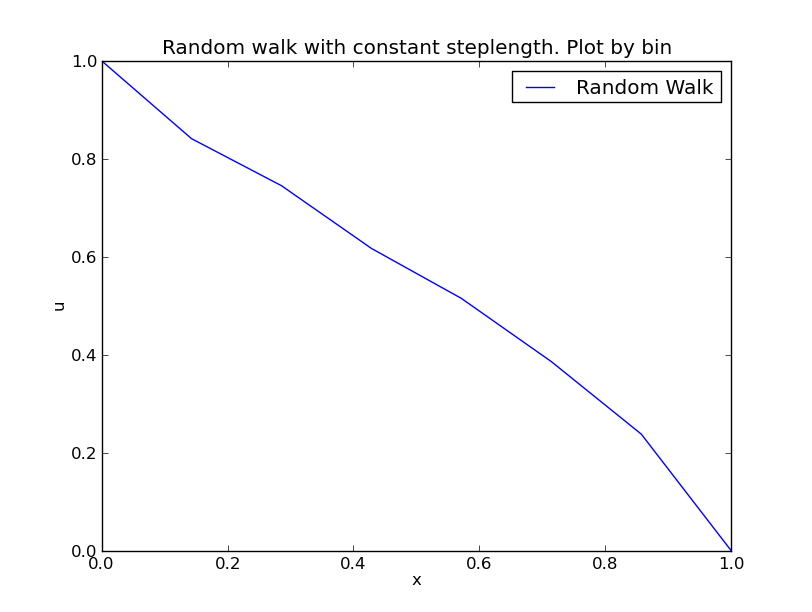
\includegraphics[width=0.55\textwidth]{build-main-Desktop-Debug/MC_uniform.png}{\centering}
  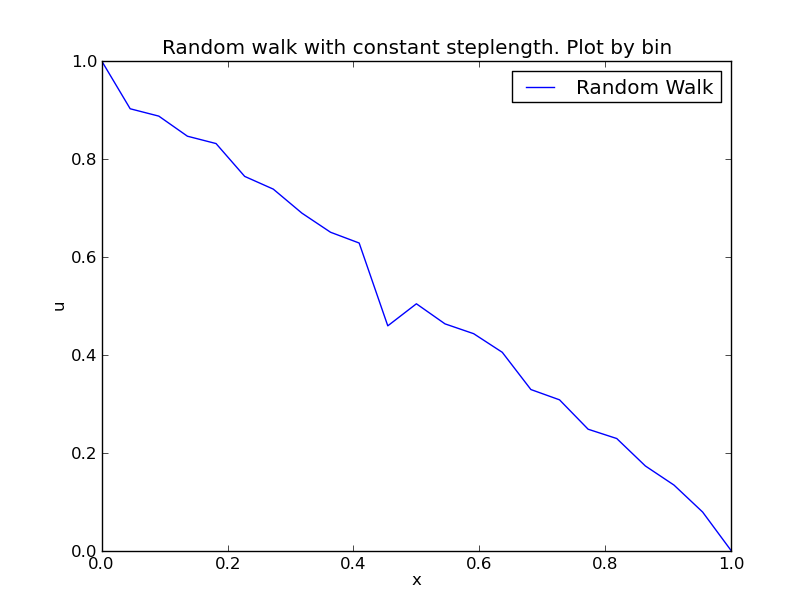
\includegraphics[width=0.55\textwidth]{build-main-Desktop-Debug/MC_uniform_low_dt.png}{\centering}
  
  In both cases, the amount of particles at position 0 are 1000. Exactly as I wanted it to be. Although
  the solutions are not very smooth, they respect the boundary conditions perfectly.
  
  When looking at the Markov chain with randomly generated steplength, I must be a little careful with
  the boundary condition at $x = 0$. I must already here decide the bin size, and make all particles within
  the first bin be equal to 1000. Not only particles with value $0$. 
  I want to make 20 bins, So all particles within $0 + \frac{1}{20} $ are counted as particle at boundary,
  and this amount cannot exceed 1000. 
  
  I will need to map the uniform random distribution to the normal distribution. The normal distribution
  looks like 
  \beq f(x) = \f{1}{\sigma \sqrt{2\pi}} e^{-\f{(x-\mu)^2}{2\sigma ^2}} \eeq
  In our case $\mu = 0$ and $\sigma = \frac{1}{\sqrt{2}}$ so we get:
  \beq f(x) = \f{1}{\sqrt{\pi}} e^{-x^2} \eeq
  So we have our new probability distribution \beq \f{1}{\sqrt{\pi}} e^{-y^2} dy = dx \eeq
  but we cannot perform the following integral analytically. \beq \f{2}{\sqrt{\pi}} \int_0^{\infty} e^{-y^2} dy = x \eeq 
  
  To get around this, I look at a distribution dependent on two uniform generated numbers.
  \beq f(y,z) = \f{1}{\sqrt{\pi}} e^{-(y^2 + z^2)} \eeq 
  Changing to polar coordinates with
  \beq r = \sqrt{y^2 + z^2} \;\;\; \theta = tan^{-1}\f{x}{y} \eeq 
  giving \beq f(r,\theta) = \f{1}{\sqrt{\pi}} r e^{-r^2} drd\theta \eeq 
  $\theta$ can be gotten by multiplying a random number by $2\pi$. To find r, we must change variables and 
  use that for exponential distribution, the mapping will look like $y(x) = -ln(1-x)$
  Set $ u = r^2$ and defining a new PDF: $e^{-u}du$. Now we see that 
  \beq y = rcos(\theta) = \sqrt{u} cos(\theta) = \sqrt{-ln(1-y')}cos(\theta) \eeq
  \beq z = rsin(\theta) = \sqrt{u} sin(\theta) = \sqrt{-ln(1-z')}sin(\theta) \eeq
  Where $y'$ and $z'$ are random numbers from uniform distribution. 
  
  This gives the following plots. First for $dt = 0.01$ and then for $dt = 0.001$
  
  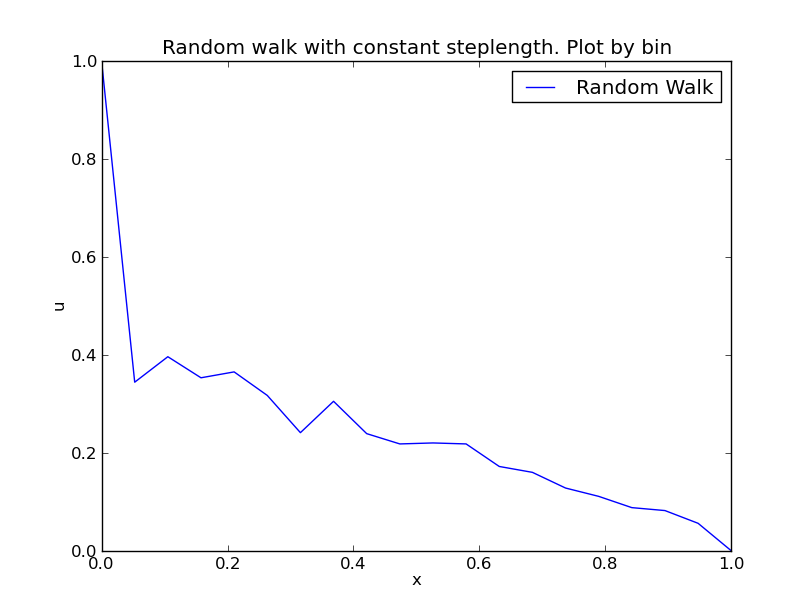
\includegraphics[width=0.55\textwidth]{build-main-Desktop-Debug/MC_normal.png}
  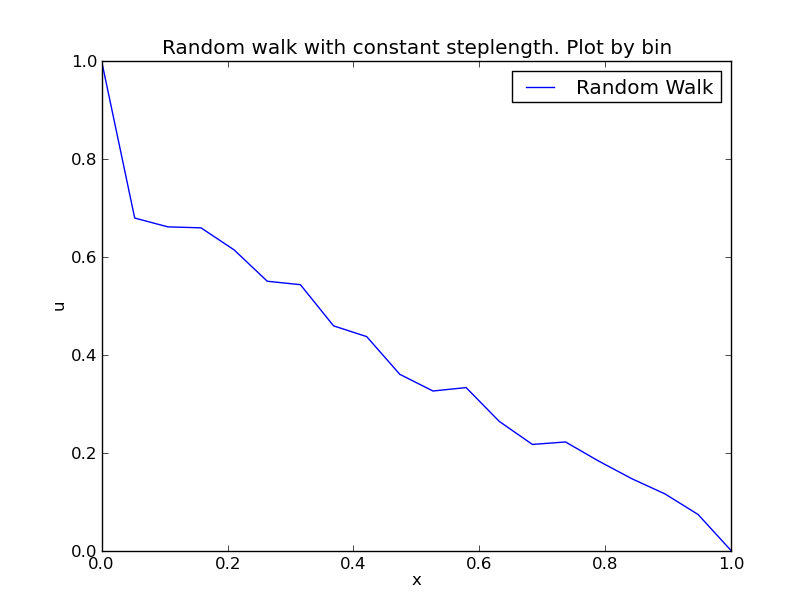
\includegraphics[width=0.55\textwidth]{build-main-Desktop-Debug/MC_normal_low_dt.png}
  which actually gives worse results than the constant steplength. 
  
  By reducing dt even further I get the following results. Left $dt = 0.0001$ and right $dt = 0.00001$:
  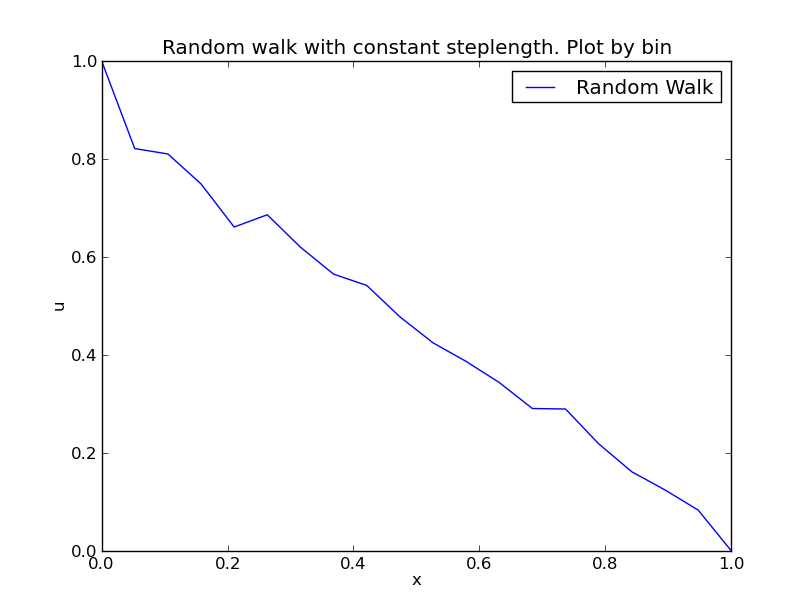
\includegraphics[width=0.55\textwidth]{build-main-Desktop-Debug/MC_normal_very_low_dt.png}
  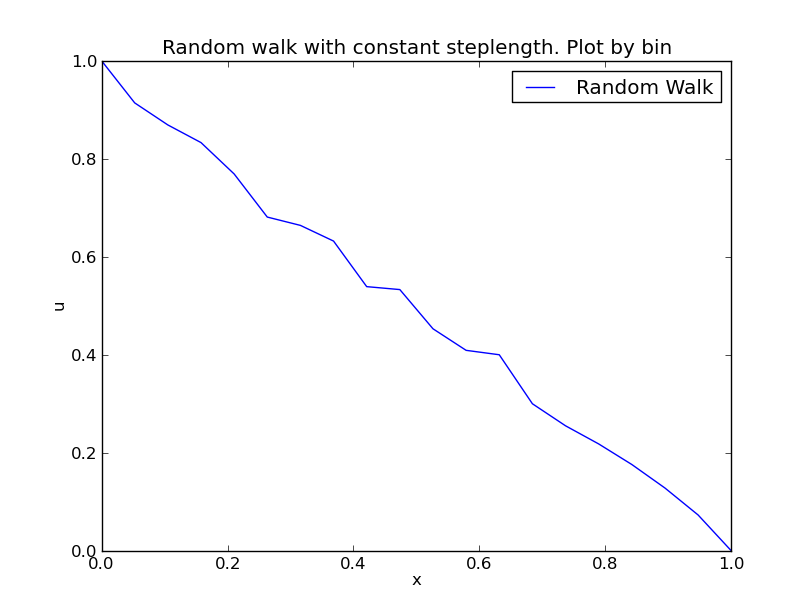
\includegraphics[width=0.55\textwidth]{build-main-Desktop-Debug/MC_normal_very_very_low_dt.png}
  
  And this is starting to look more like the analytic / Crank Nicolson solution, even though it is
  still not too smooth.  For $dt = 0.00001$, the computer needed 177 seconds, so this is starting to demand
  resources. 
  
  \end{subsection}
  \begin{subsection}*{Crank Nicolson}
   I solve the equation numerically using Crank Nicolson to compare with the Markov Chains. By setting 
   $dx = 0.01$ and $dt = 0.01$ (the same values as for Markov Chain with constant steplength), I get the
   following results. The right plot shows the first 3 timesteps, one get a feeling how it evolvs in time. 
   (blue: t0, red t1, green t2)
   
   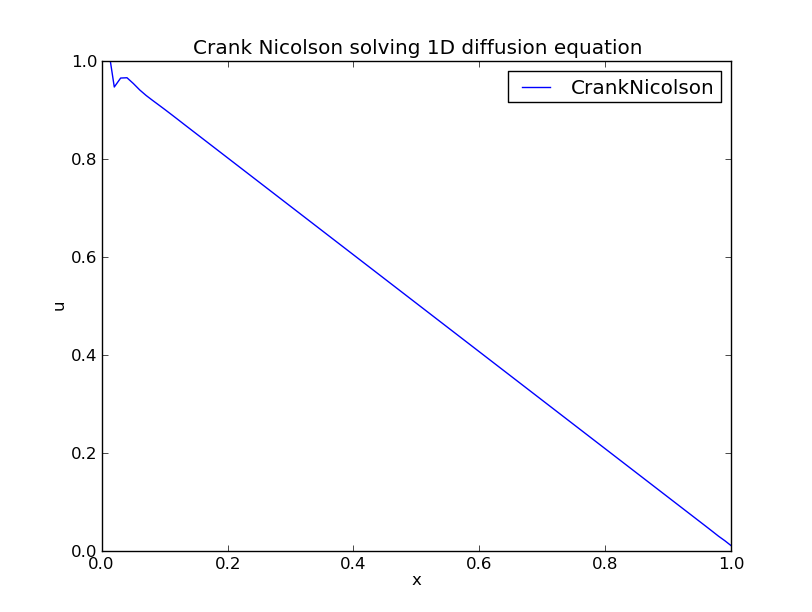
\includegraphics[width=0.55\textwidth]{build-main-Desktop-Debug/CrankNicolson.png}{\centering}
   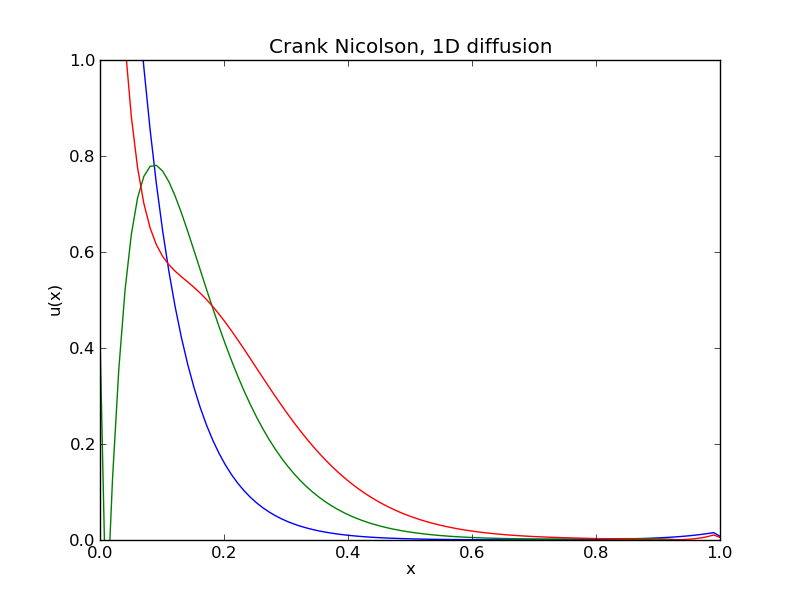
\includegraphics[width=0.55\textwidth]{build-main-Desktop-Debug/CrankNicolson_first3.png}{\centering}
   
   Decreasing $dt$ by a factor $10^3$ for Crank Nicolson and by a factor $10$ for the random walk, 
   one can see the difference in efficiency for these two methods. The random walk method used 7 seconds, 
   while the Crank Nicolson scheme used 6 seconds. Which is clearly in favour of Crank Nicolson since $dt$
   was reduced much more. For these values,
   Crank Nicolson gives very high accuracy, while the Random walk method do not show significant improvements.
   Plots below:
   
   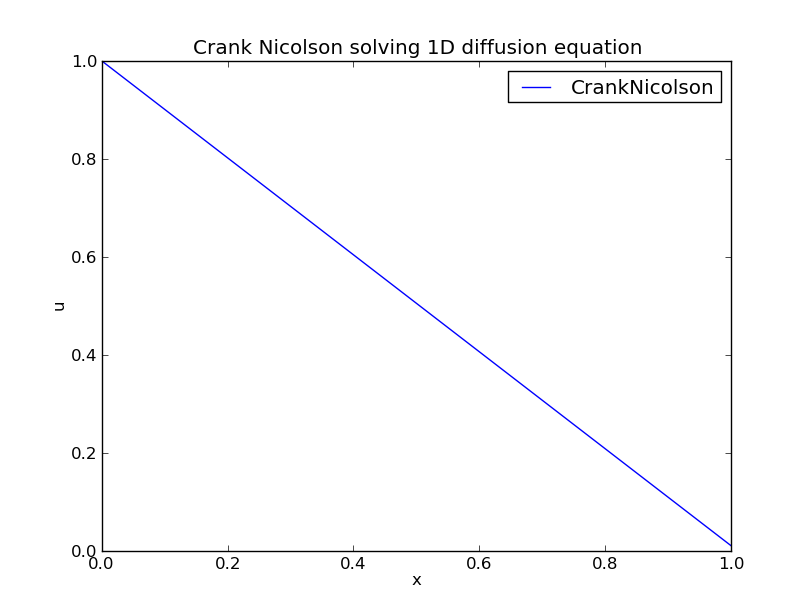
\includegraphics[width=0.55\textwidth]{build-main-Desktop-Debug/CrankNicolson_low_dt.png}
   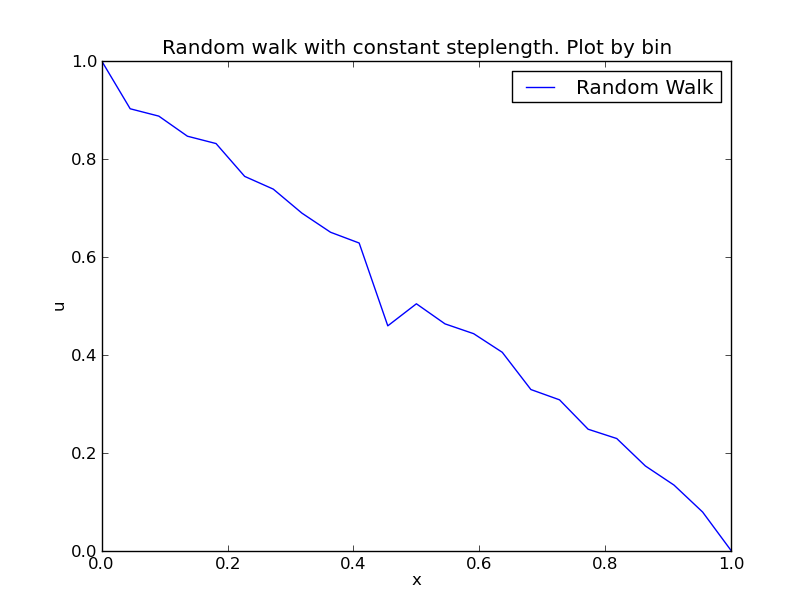
\includegraphics[width=0.55\textwidth]{build-main-Desktop-Debug/MC_uniform_low_dt.png}
   
  \end{subsection}

 \end{section}
    
 
 \begin{section}*{Analytical solution of 2+1 dimensional problem} 
  We have seen before that the solution of a 1+1 dimensional problem is 
  \beq u(x,t) = \sum_{n=1}^{\infty} \f{-2}{\pi n} sin(n\pi x) e^{-n^2\pi ^2 t} + x - 1 \eeq
  To find the solution for the 2+1 dimensional problem, I will use separation of variables for both
  $X(x)$, $Y(y)$ and $T(t)$. I need boundary conditions for $X$ and $Y$ and initial condition for $T$.
  The boundary conditions for $X$ are given as \beq u(0,y,t) = 1, \;\;\; u(1,y,t) = 0 \eeq
  The initial condition is given as
  \beq u(x,y,0) = 0, \;\; 0 < x < 1 \eeq
  The boundary conditions for the Y-direction is not given, so I have to set them for myself. Since the 
  synaptic cleft is finite and we only want the ions inside the cleft, the concentration of ions must
  be reduced to 0 in the y-direction, so a guess for boundary conditions might be 
  \beq u(x,0,t) = u(x,1,t) = 0 \eeq
  
  The y-direction is along the synapses, and the x-direction is perpendicular to the synapses. So the 
  density is highest at $x=0$ and will be reduced as $x$ increases. X-direction is the same as for the 
  1dimension system.
  \begin{subsection}*{Finding steady state solution}
  I need the steady state solution for my problem, and that is given by solving the Laplace equation:
  \beq \nabla ^2u_s = 0\eeq
  by separation of variables that reduces to:
  \beq \frac{1}{X(x)} \frac{d ^2 X(x)}{d x^2} = \lambda ^2 \;\; \frac{1}{Y(y)} \frac{d^2Y(y)}{dy^2} = -\lambda ^2\eeq
  And I get the solutions:
  \beq Y(y) = \alpha cos(\lambda y) + \beta sin(\lambda y) \;\; X(x) = \gamma cosh(\lambda x) + \delta sinh(\lambda x) \eeq
  Need to check boundary conditions to solve the unknown variables. 
  \beqq u_s(0,y) = 1 = \gamma(\alpha cos(\lambda y) + \beta sin(\lambda y)) \eeqq
  \beqq u_s(x,0) = 0 = \alpha(\gamma cosh(\lambda x) + \delta sinh(\lambda x)) \eeqq
  So we see that for these equations to hold, (without resorting to the non-trivial solution), $\alpha = 0$ 
  and therefore \beq \gamma \beta sin(\lambda y) = 1 \eeq
  \beqq  u_s(x,1) = 0 = \beta sin(\lambda) [\gamma cosh(\lambda x) + \delta sinh(\lambda x)] \eeqq
  Since $\beta = 0$ leads to a nontrivial solution, we must set $sin(\lambda) = 0$. That leads to 
  \beq \lambda = n\pi \;\;\; n = 1,2,3,... \eeq 
  The last equation 
  \beqq u_s(1,y) = 0 = \beta sin(n\pi y) [\gamma cosh(n\pi) + \delta sinh(n\pi)] \eeqq
  leads to \beq \gamma cosh(n\pi) = -\delta sinh(n\pi) \eeq
  \beq \delta = -\gamma coth(n\pi) \eeq 
  
  To find out the solution for (2):
  \beq 1 = \gamma \beta sin(n\pi y) \eeq
  I must use Fourier expansion theory:
  \beq 1 = \sum_{n=1}^{\infty} \gamma_n sin(n\pi y) \;\;\;\; \gamma_n = 2\int_0^1 sin(n\pi y) dy \eeq 
  \beq \gamma_n = \frac{2}{n\pi}(1 - cos(n\pi)) \eeq 
  
  Now I can put everything back together, and I find that
  \beq u_s(x,y) = \beta sin(n\pi y) [\gamma cosh(n\pi x) - \gamma coth(n\pi) sinh(n\pi x)] \eeq
  Leading to the final solution
  \beqq u_s(x,y) = \sum_{n=1}^{\infty} \frac{2}{n\pi}(1-cos(n\pi)) sin(n\pi y) [cosh(n\pi x) - coth(n\pi) sinh(n\pi x)] \eeqq
  
  By plotting the steady state solution, I can see what the diffusion equation will converge towards, and 
  I can compare this plot to the explicit and the implicit scheme. I only plot what the concentration looks
  like after a long time, so the schemes should have converged towards the steady state solution.
  
  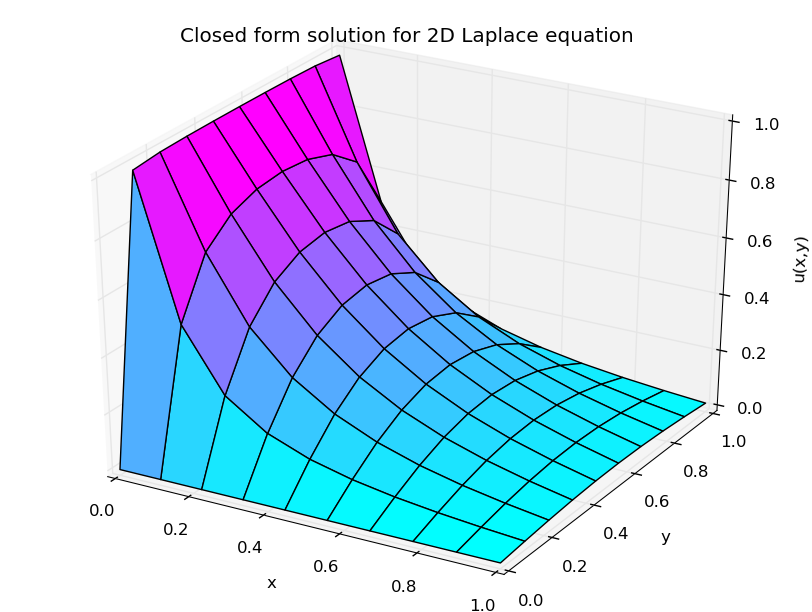
\includegraphics[width=0.8\textwidth]{build-main-Desktop-Debug/SteadyState.png}
 
  \end{subsection}
  
  \begin{subsection}*{Analytic 2+1D diffusion}
   Now, let's try to solve the 2D diffusion equation! 
   
   First, we separate variables:
   \beq \f{1}{X(x)} \f{\pa^2 X(x)}{\pa x^2} + \f{1}{Y(y)} \f{\pa^2 Y(y)}{\pa y^2} = \f{1}{T(t)} \f{\pa T(t)}{\pa t}\eeq 
   
   which gives the time solution \beqq T(t) = e^{-\lambda ^2 t} \eeqq
   and the following spacial equation
   \beq \f{1}{X(x)} \f{\pa^2 X(x)}{\pa x^2} = -\lambda ^2 - \f{1}{Y(y)} \f{\pa^2 Y(y)}{\pa y^2} \eeq
   Again, each of these have to be constant:
   \beq \f{1}{X(x)} \f{\pa^2 X(x)}{\pa x^2} = \rho ^2 = -\lambda ^2 - \f{1}{Y(y)} \f{\pa^2 Y(y)}{\pa y^2} \eeq
   We get the solutions
   \beq X(x) = \gamma cosh(\rho x) + \delta sinh(\rho x) \;\;\;
   Y(y) = \alpha cos(\rho y) + \beta sin(\rho y) + \sigma cos(\lambda y) + \theta sin(\lambda y) \eeq
   
   Inforcing the boundary conditions:
   \beq u(0,y) = 1 = \gamma (\alpha cos(\rho y) + \beta sin(\rho y) + \sigma cos(\lambda y) + \theta sin(\lambda y)) \eeq
   \beq u(x,0) = 0 = (\alpha + \sigma) (\gamma cosh(\rho x) + \delta sinh(\rho x)) \eeq
   Setting $\alpha = -\sigma$ to solve this equation. 
   \beq u(x,1) = 0 = (\gamma cosh(\rho x) + \delta sinh(\rho x)) (\alpha cos(\rho)+\beta sin(\rho )-\alpha cos(\lambda)+\theta sin(\lambda )) \eeq
   By setting $\alpha = 0$, I can get $\rho = \lambda = n\pi$. This is not a general solution, but the 
   steady state solution I already have calculated. Without making any such breathtaking assumptions, I have
   too few boundary conditions to solve this problem by separation of variables. 
   
   Although I can not solve this diffusion equation, the steady state solution will serve it's purpose, since
   I compare plots after enough time has passed for the soltion to converge to the steady state. 
  
  \end{subsection}
  
  \end{section}

  \begin{section}*{2+1 dimensional problem. Numerical solution}
  
  \begin{subsection}*{Explicit method}
    I will use two different schemes to simulate the 2-dimensional diffusion equation. First I will look at 
    the explicit scheme and its stability. 
    
    The algorithm is pretty straight-forward 
    \beq u_{i,j}^{l+1} = u_{i,j}^l + \alpha[u_{i+1,j}^l + u_{i-1,j}^l + u_{i,j+1}^l + u_{i,j-1}^l - 4u_{i,j}^l] \eeq
    which is derived by applying the numerical approximation for the double derivative and reorganizing the
    equation. $\alpha = \frac{\Delta t}{h^2} $ The scheme is explicit because it generates the value at the 
    next time step based on the previous time step. 
    
    For the 1 dimensional explicit scheme, we had problems with stability if $\Delta t > \f{1}{2}\Delta x^2$
    For the two-dimensional case, I found that at $\Delta x = 0.1$ and $\Delta t = 1/370 = 0.0027$, the 
    explicit scheme stabalized. This is barely more than $\f{1}{4}\Delta x^2$, so based on this, I say that
    \beq \Delta t \geq \f{1}{4} \Delta x^2 \eeq 
    If we want a stable solution. 
    Following are four plots of the explicit solution: 
    
    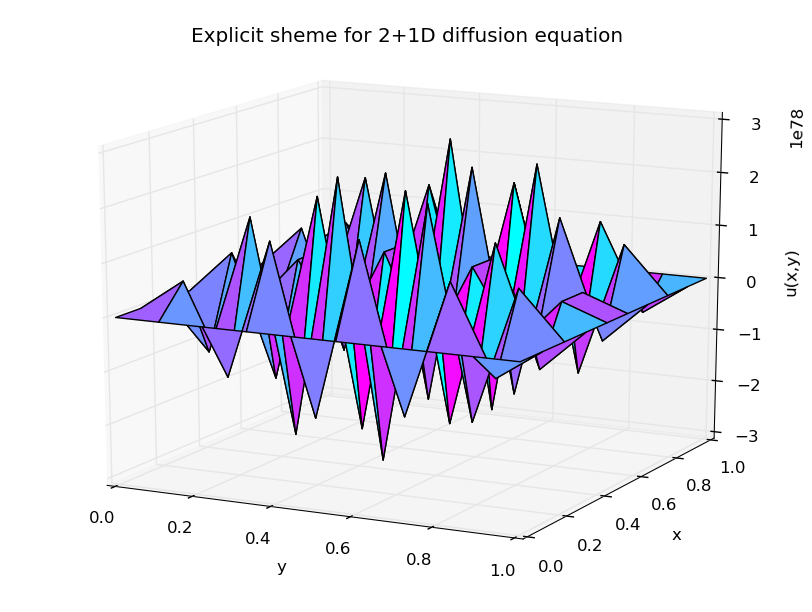
\includegraphics[width=0.55\textwidth]{build-main-Desktop-Debug/Explicit100.png}
    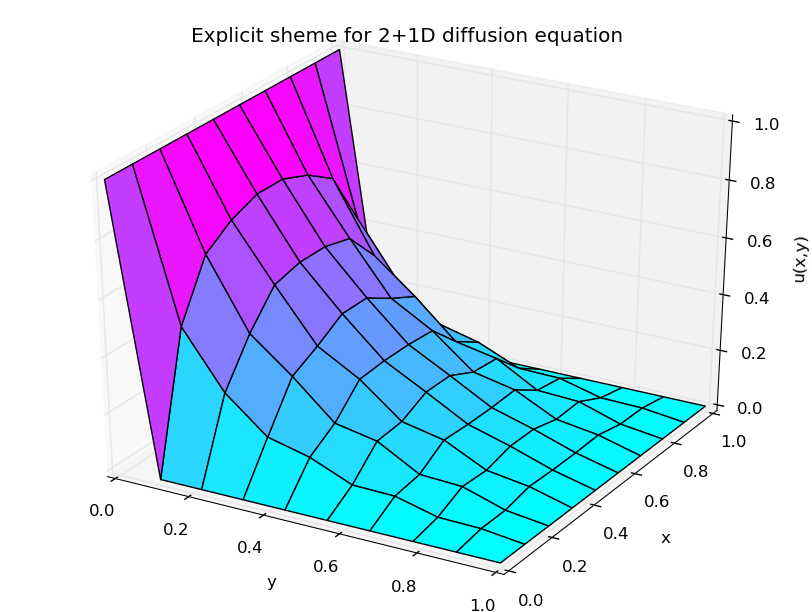
\includegraphics[width=0.55\textwidth]{build-main-Desktop-Debug/Explicit369.png}
    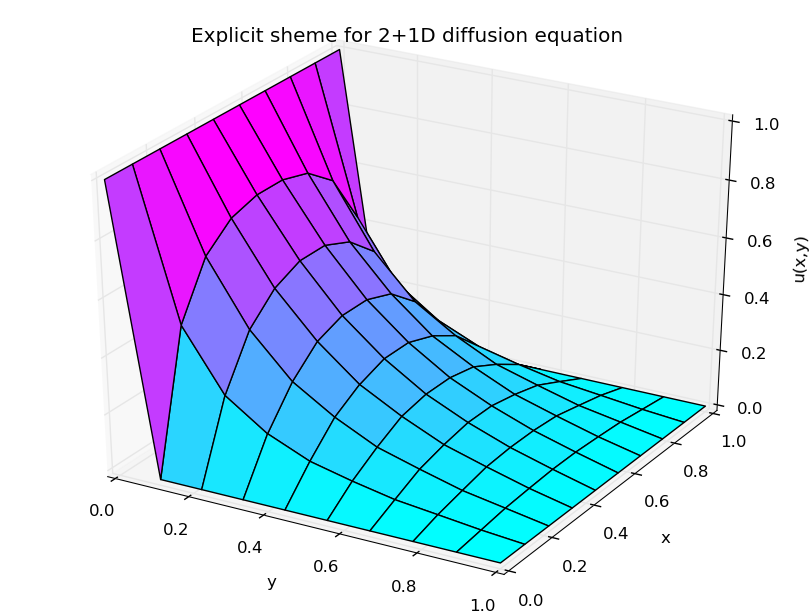
\includegraphics[width=0.55\textwidth]{build-main-Desktop-Debug/Explicit370.png}
    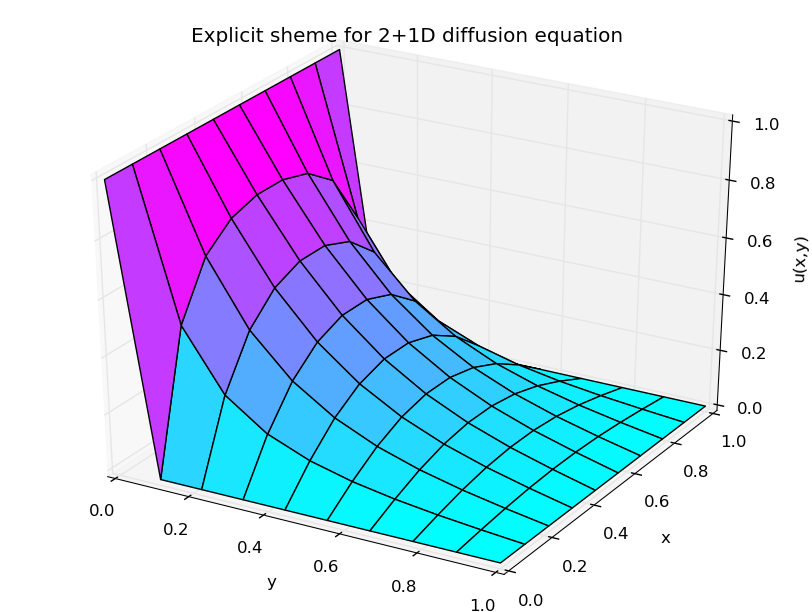
\includegraphics[width=0.55\textwidth]{build-main-Desktop-Debug/Explicit1000.png}
    
    Top left: $dt = \f{1}{100}$, top right: $dt = \f{1}{369}$, lower left: $dt = \f{1}{370}$,
    lower right $dt = \f{1}{1000}$
    
    The results I get from the explicit scheme is close to the analytic steady state solution. 
    
 \end{subsection}
  \begin{subsection}*{Implicit method}
   The implicit method is derived almost identically as the explicit scheme, but one uses the backward going
   Euler formula instead of the forward going formula for the time derivative on the diffusion equation.
   Reorganizing the equation, I end up with
   \beq u_{i,j}^l + 4\alpha u_{i,j}^l - \alpha[u_{i+1,j}^l + u_{i-1,j}^l + u_{i,j+1}^l + u_{i,j-1}^l] = u_{i,j}^{l-1} \eeq
   Which is an equation that has many unknown values at time $l$ that are decided from a single point at
   an earlier time, $l-1$. 
   
   The way I solve this equation is by using Jacobi's method. I guess an initial $u$, then computing a new 
   solution $u_{new}$ by the given equation, and then I see if my new solution $u_{new}$ is close enough to 
   my initial guess $u$. If yes: Then I have a good enough solution. If not: then I set $u = u_{new}$ and 
   compute $u_{new}$ again, based on the revised u. 
   
   This scheme has no stability issues like the explicit scheme has. The error is the same as for the 
   explicit scheme, since the backward and the forward Euler formula has the same error, but since I do
   not have to worry about the stability, I can increase the spacial resolution quite a bit without my 
   results going bananas! 
   
    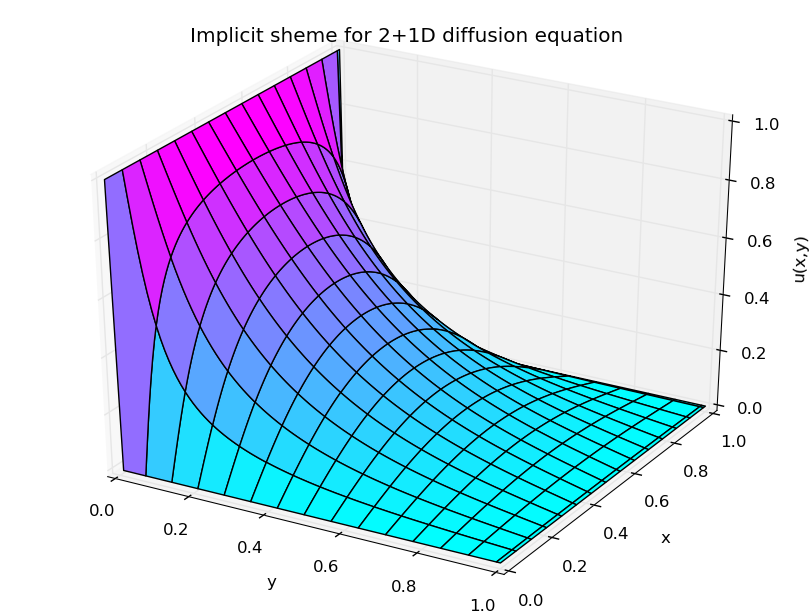
\includegraphics[width=0.55\textwidth]{build-main-Desktop-Debug/Implicit100_100.png}
    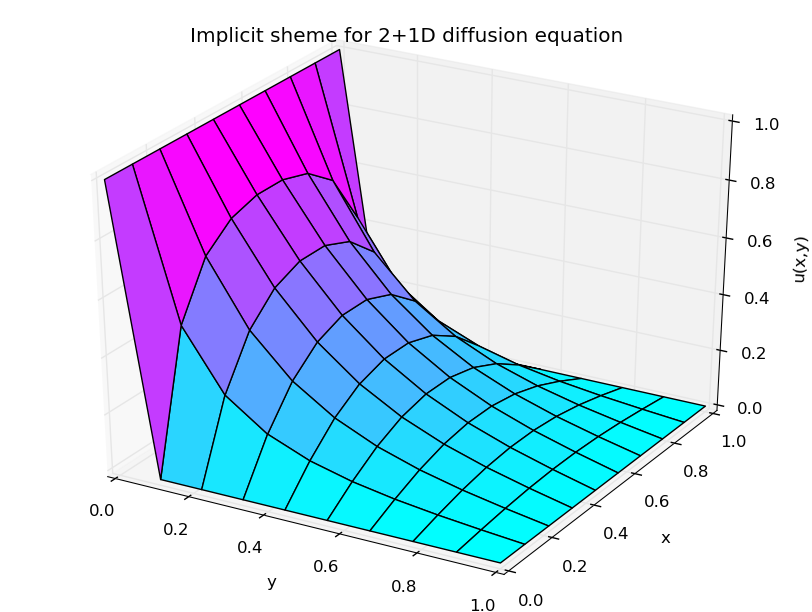
\includegraphics[width=0.55\textwidth]{build-main-Desktop-Debug/Implicit10_1000.png}
    
   First plot has a $\Delta x = 0.01$ and $\Delta t = 0.01$. This made the explicit scheme unstable, but
   I could with no problem get a higher spacial resolution here without decreasing the time step.
   Second plot has $\Delta x = 0.1$ and $\Delta t = 0.001$. This looks exactly equal to the explicit 
   solution, which would be natural. It also looks very close to the closed form solution for the steady state.
   
   As a final comparison, I have rotated the plots, so I can see them from the side. Here it becomes quite 
   obvious that the numerical schemes have a noticable error. Both the implicit and the explicit scheme
   goes to 0 way too fast! 
   
   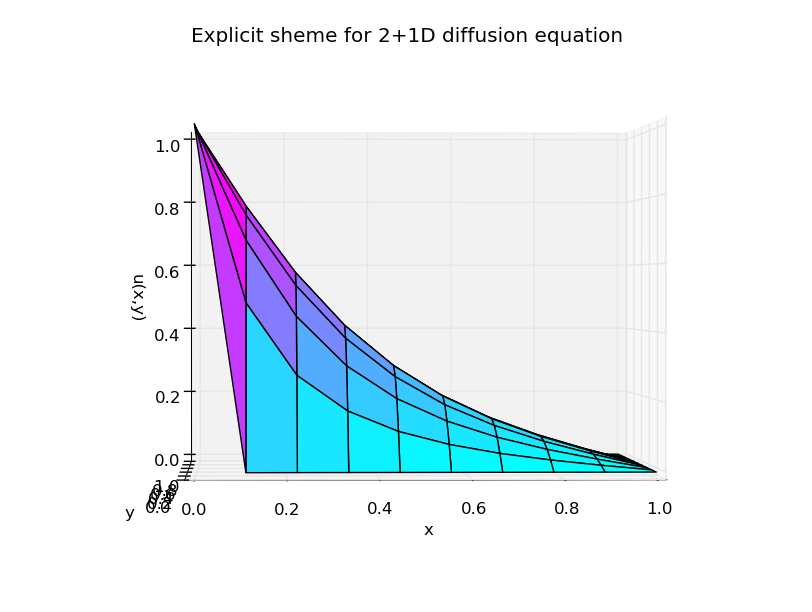
\includegraphics[width=0.55\textwidth]{build-main-Desktop-Debug/Explisit_side.png}
   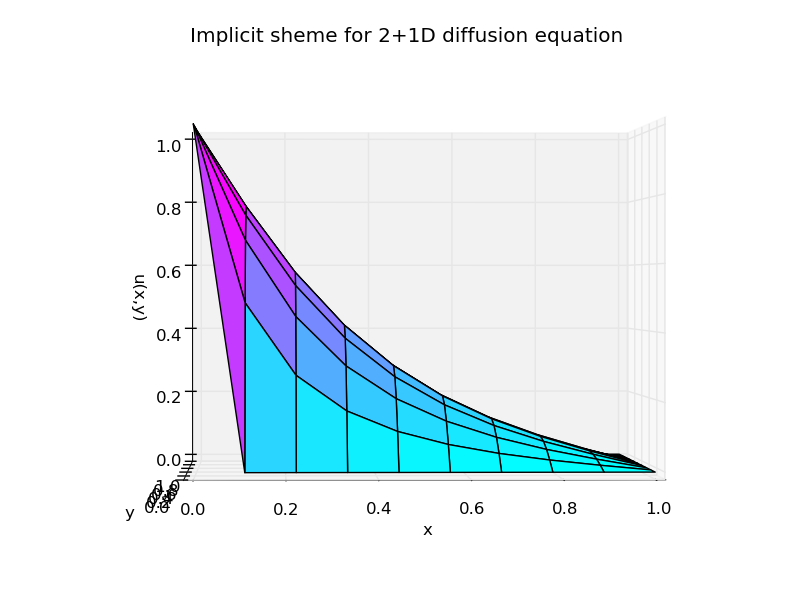
\includegraphics[width=0.55\textwidth]{build-main-Desktop-Debug/Implicit_side.png}
   
   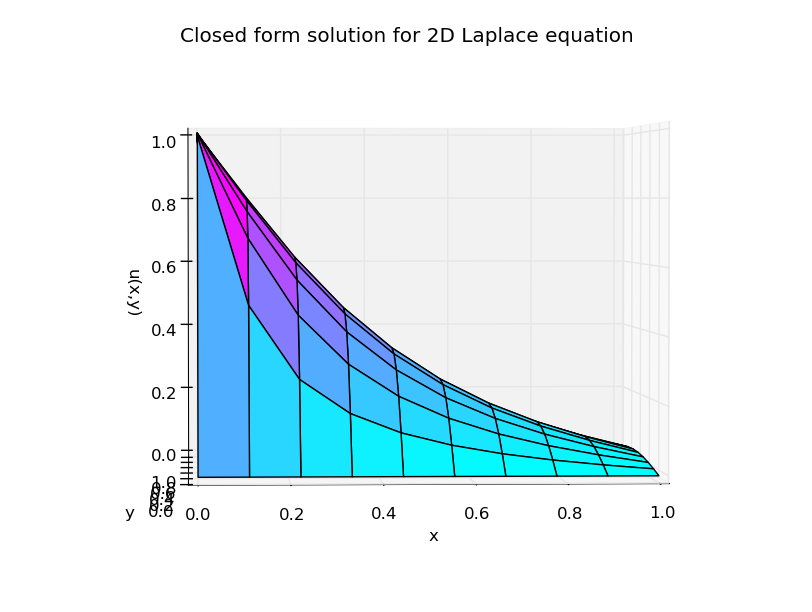
\includegraphics[width=0.6\textwidth]{build-main-Desktop-Debug/Analytic_side.png}
   \end{subsection}

  \end{section}
  
\end{document}
